\documentclass[11pt]{article}
    \usepackage{caption}
    \usepackage{graphicx}
    \usepackage{mathtools}
    \usepackage{bookmark}
    \setlength{\parindent}{0pt}
    \DeclareCaptionType{equ}[][]
    \usepackage[svgnames]{xcolor}
    
    \newcommand*{\plogo}{\fbox{$\mathcal{BM}$}}
    
    \usepackage{PTSerif}
    
    \begin{document} 
        
    \begin{titlepage}
    
        \raggedleft
        
        \vspace*{\baselineskip}
        
        {\Large Bryan Melanson}
        
        \vspace*{0.167\textheight}
        
        \textbf{\LARGE How to Not Fail}\\[\baselineskip]
        
        {\textcolor{Red}{\Huge Control Systems}}\\[\baselineskip]
        
        {\Large \textit{While never going to class}}
        
        \vfill
        
        {\large Computer Engineering 2020 ~~\plogo}
        
        \vspace*{3\baselineskip}
    
    \end{titlepage}

    \pagebreak
    
    \pdfbookmark[section]{\contentsname}{toc}

    \tableofcontents

    %%%%%%%%%%%%%%%%%%%%%%%%%%%%%%
    
    \section{Modelling}
    
    %%%%%%%%%%%%%%%%%%%%%%%%%%%%%%

    \section{Time Response}
    
    %%%%%%%%%%%%%%%%%%%%%%%%%%%%%%
    
    \section{Systems Reduction}

    %%%%%%%%%%%%%%%%%%%%%%%%%%%%%%

    \section{Stability}

    Mathematically, stability for linear, time-invariant systems can be determined from the location of the closed-loop poles:

    \begin{itemize}
        \item{If the poles are only in the left half-plane, the system is stable.}
        \item{If any poles are in the right half-plane, the system is unstable.}
        \item{If the poles are on the j$\omega$ axis and in the left half plane, the system is marginally stable as long as the poles on the j$\omega$ axis are of unit multiplicity; it is unstable if there are any multiple j $\omega$ poles.}
    \end{itemize}
    

    \subsection{Routh Hurwitz}

    The \textit{Routh-Hurwitz criterion} lets us find how many poles are in each section of the s-plane without giving us the coordinates of the poles. Just knowing that there are poles in the right half-plane is enough to determine that a system is unstable. Under certain limited conditions, when an even polynomial is present, the Routh table can be used to factor the system’s characteristic equation.
    \begin{center}
        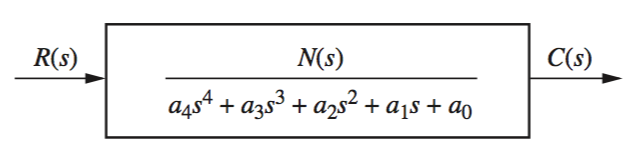
\includegraphics[width = 300 px]{img/routh-t}        
    \end{center}
    \begin{center}
        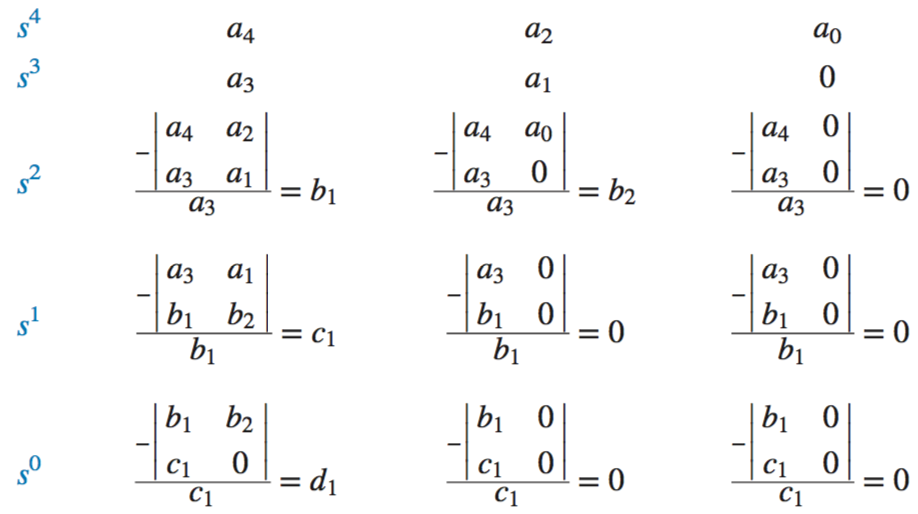
\includegraphics[width = 300 px]{img/routh}        
    \end{center}

    \begin{center}
        \textbf{Recall} - $det = (a_1 \cdot b_2) - (a_2 \cdot b_1)$
    \end{center}
    \subsubsection{Zero Only in First Column}
    \begin{center}
        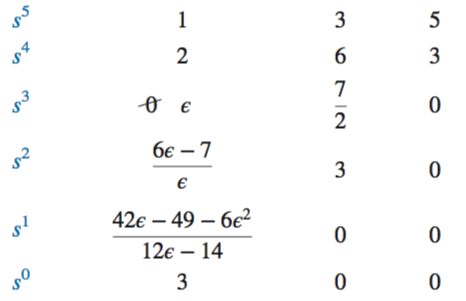
\includegraphics[width = 300 px]{img/routh-e}        
    \end{center}
    \begin{center}
        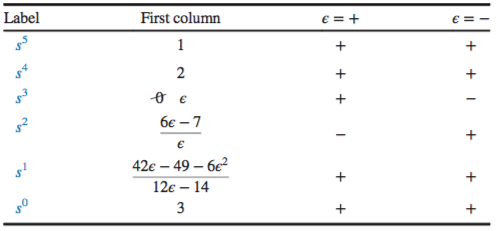
\includegraphics[width = 300 px]{img/routh-e2}        
    \end{center}
    \subsubsection{Entire Row of Zeroes}
    \subsubsection{Reverse Coefficients}
    \begin{center}
        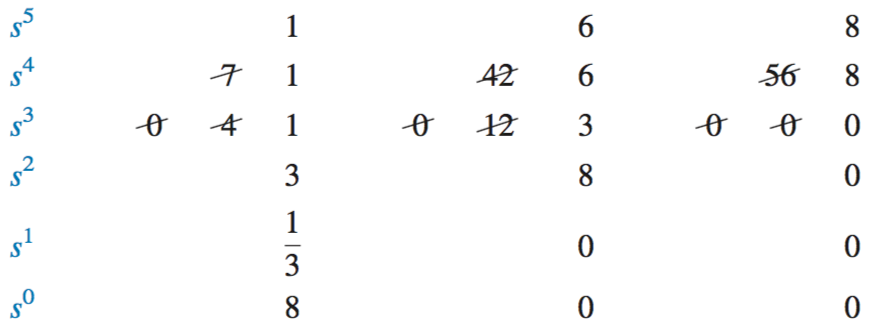
\includegraphics[width = 300 px]{img/routh-roz}        
    \end{center}
    \subsection{Stability in State Space}

    %%%%%%%%%%%%%%%%%%%%%%%%%%%%%%

    \section{Steady State}

    %%%%%%%%%%%%%%%%%%%%%%%%%%%%%%

    \section{Root Locus}

    %%%%%%%%%%%%%%%%%%%%%%%%%%%%%%

    \section{Root Locus Design}

    %%%%%%%%%%%%%%%%%%%%%%%%%%%%%%

    \section{Frequency Response}

    %%%%%%%%%%%%%%%%%%%%%%%%%%%%%%

    \section{Digital Control}

    %%%%%%%%%%%%%%%%%%%%%%%%%%%%%%

    \end{document}